\documentclass{beamer}
%\documentclass[handout,t]{beamer}

\batchmode
% \usepackage{pgfpages}
% \pgfpagesuselayout{4 on 1}[letterpaper,landscape,border shrink=5mm]

\usepackage{amsmath,amssymb,enumerate,epsfig,bbm,calc,color,ifthen,capt-of}
\usepackage[all]{xy}

\usetheme{Boadilla}
\usecolortheme{mit}

\title{Blockchain Overview}
\author{Darren Tapp}
\date{August 22, 2018}

\institute[]{MIT Alumni Club of NH}


%\beamerdefaultoverlayspecification{<+->}
% -----------------------------------------------------------------------------
\begin{document}
% -----------------------------------------------------------------------------

\frame{\titlepage}

  

\begin{frame}{About Me}

  About Darren Tapp:

  \begin{itemize}
    \item Lead researcher at DASH (Digital Cash)
    \item Developing a blockchain course for Arizona State University
    \item Mathematician by training    
  \end{itemize}

\end{frame}


\begin{frame}{Definition}

\begin{block}{What is a Blockchain?}
A blockchain is a sequence of \emph{blocks} that are \emph{chained} together that provide instructions on how to change information we will call the \emph{global state}.

A blockchain must allow any two observers (most likely computers) to agree on a global state, possibly after an exchange of blocks.
\end{block}

\pause

There is not a clear definition in the literature.

  
\end{frame}




\begin{frame}{What is a Block?}
  \vfill

  \begin{block}{What is a Block?}
    A block is data.  The data include a block header and messages.
  \end{block}

\vfill
  

\[  
  \xymatrix{
  *+[F]{\txt{Block Header}} \ar@{<.>}[d]\\
  *+[F]{\txt{Message 1 \\ Message 2 \\ \vdots} }} 
\]


\vfill

\end{frame}

\begin{frame}{Chain?}


  \begin{block}{What Is Meant by Chain?}
    Each block header has a digital fingerprint, called a hash, of the previous block.
  \end{block}
  \[
  \xymatrix{
    \ar[r] &  *+[F]{\txt{Block Header \#5\\ Fingerprint of \#4 
     }} \ar[r] & *+[F]{\txt{Block Header \#6\\ Fingerprint of \#5 
     }}  \ar[r]& *+[F]{\txt{Block Header \#7\\ Fingerprint of \#6 
     }} }
  
  \]

\end{frame}


\begin{frame}{Global State}
  \begin{iteize}
  \item The messages usually are instructions for updating the global state.  
  \end{itemize}


\[  
  \xymatrix{
    *+[F]{\txt{Block Header}} \ar@{<.>}[dd]\\
      & *+[F]@*[o]{\txt{$\star$\\Global \\State\\$\star$}} \\
    *+[F]{\txt{Message 1 \\ Message 2 \\ \vdots} } \ar[ur]^{update}} 
\]  
\end{frame}



\begin{frame}{Design Properties}


\begin{block}{First Design Property}
  It is intentionally difficult to find the next block.

  It generally takes all participating computers $\ldots$ 
  \pause
  \begin{itemize}
    \item $10$ minutes to find the next block on Bitcoin
    \item $2\frac{1}{2}$ minutes to find the next block on Dash
  \end{itemize}

\end{block}

\pause
  
  \begin{block}{Second Design Property}
    In the event of more than one chain, the chain that is most difficult to create is considered valid.
  \end{block}
  
\end{frame}


\begin{frame}{An Orphan Block}


   \[
  \xymatrix{
    \ar[r] &  *+[F]{\txt{Block Header \#6\\ Fingerprint of \#5 
     }} \ar[r] \ar[dr]& *+[F]{\txt{Block Header \#7a\\ Fingerprint of \#6 
     }}  \ar[r] & *+[F]{\txt{Block Header \#8\\ Fingerprint of \#7a 
     }} \\ & & *+[F]{\txt{Block Header \#7b\\ Fingerprint of \#6 
     }}}
  
  \]
  \pause
  Block 7b will most likely be orphaned. \\
  \pause
  Messages in 7b do not update the global state unless they are included in block 7a, or 8, etc.

\end{frame}

\begin{frame}{Third Design Property}
  \begin{block}{Third Design Property}
    The Merkle root of all messages included in that block
    is added to the block header.  This allows for an efficient cryptographic
    proof that a message is in a block.
  \end{block}

\end{frame}

\begin{frame}{Merkle Tree}

\begin{center}
  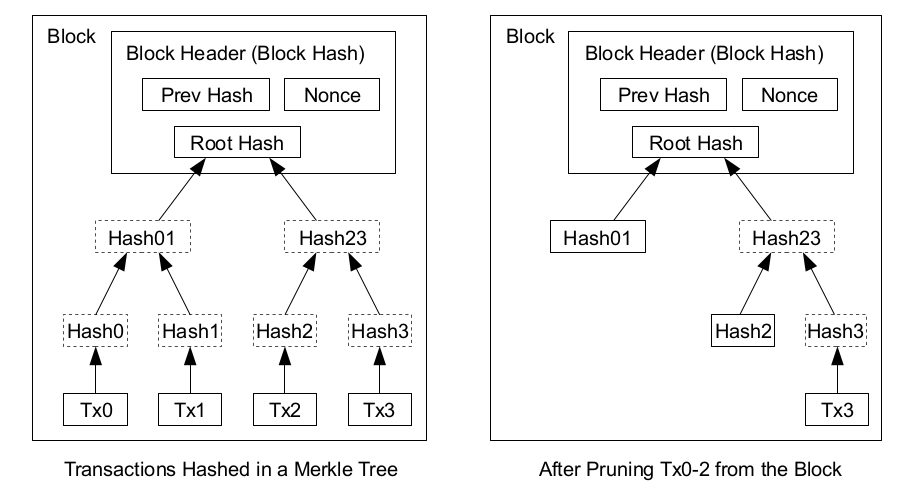
\includegraphics[height=2in]{MerkleTree.png}
\end{center}

  
\end{frame}



\begin{frame}{End Product}

In my view:
  
  \begin{block}{End Product}
    The end product is a decentralized governance.  If a block is submitted to the network that does not enforce
    given rules, it will be rejected and orphaned.
  \end{block}

\pause
  
  \begin{block}{By-product}
    A by-product of this setup is that a record is created that is difficult to change.
  \end{block}

  
\end{frame}

\begin{frame}{Stable Governance?}

  \begin{block}{Stable Nash Equilibrium}
    Done correctly, a blockchain provides governance that operates at a stable Nash equilibrium.
  \end{block}

  \pause

  \begin{block}{General English Translation}
    It is more profitable to enforce the protocol than to attack it.
  \end{block}

\end{frame}

\begin{frame}{Applications}
  Working experimental applications:
  \begin{itemize}
    \item Currency (Bitcoin Cash, Dash)
    \item Turing complete finite state machine (Ethereum)
  \end{itemize}
  
\end{frame}

\begin{frame}{Currency Application}
  \begin{block}{Currency Application}
    For the currency application:  Messages are transactions, and the global state is the set of Unspent
    Transaction Outputs.  
  \end{block}

  \[  
  \xymatrix{
    *+[F]{\texttrm{Block Header}} \ar@{<.>}[dd]\\
      & *+[F]@*[o]{\txt{$\star$\\ UTxO set \\$\star$}} \\
    *+[F]{\txt{Transaction 1 \\ Transaction 2 \\ \vdots} } \ar[ur]^{update}} 
  \]  


\end{frame}

\begin{frame}{Philosophy}
  \begin{center}
  If time allows:  Philosophy\\
  \vspace{0.5 in}
  \pause

  Synthetic Reality
  \end{center}
\end{frame}

\begin{frame}{Thank You}
  \begin{center}
  Thank you! \\
  \vspace{0.5 in}

  \pause
  
  Questions?
  \end{center}
\end{frame}

% -----------------------------------------------------------------------------
\end{document}
